\chapter{API Konzept}
\label{apikonzept}

\section{Trennung}

Um strongTNC von strongSwan zu trennen und die gemeinsame Datenbank abzulösen,
wurde im Rahmen dieser Arbeit ein API Konzept erarbeitet. Das Konzept orientiert
sich dabei am \enquote{REST} Architekturstil, welcher von Roy Fielding in seiner
Dissertation aus dem Jahr 2000 erstmals definiert
wurde\cite{fielding2000architectural}.

In diesem Abschnitt werden wichtige Punkte des API Konzeptes genauer betrachtet.
Das vollständige Konzept ist im Anhang (Abschnitt \ref{REST:api-konzept} ab
Seite \pageref{REST:api-konzept}) zu finden. Detaillierte Beschreibungen zur
verwendeten Syntax, sowie die Definition der Archetypes, sind ebenfalls im
Konzept zu finden.

\nobrsection{Vorgehen}

Das Ziel der REST API ist eine vollständige Ablösung der gemeinsamen Datenbank
als Schnittstelle. Um einen Überblick über den benötigten Umfang einer TNC
Policy Manager Schnittstelle zu bekommen, wurden die Datenbankzugriffe im IMV
Code der strongSwan Implementation betrachtet. Dazu wurden sämtliche SQL
abfragen im IMV Quellcode gesammelt und analysiert. Das Ergebnis war eine Liste
der Tabellen, auf die schreibend oder lesend zugegriffen wurde. Ebenso konnte
ermittelt werden, welche Tabelle über ein SQL \texttt{JOIN} Statement verknüpft
wurden. Basierend auf diesen Daten konnte ein Set von REST Endpunkten definiert
werden, mit dem es möglich ist, sämtliche aktuell bestehenden Datenbankzugriffe
abzudecken.

\section{Documents und Collections}

Für alle Elemente der strongTNC Domäne wurden REST Ressourcen von den Archetypes
\enquote{Document} und \enquote{Collection} konzipiert. Oft handelt es sich
dabei um vollständige CRUD Ressourcen, wie beispielsweise bei der
\texttt{Version} Ressource sichtbar ist:

\begin{listing}[H]
\caption{REST Document für Versions}
\begin{mdframed}[style=def]
\begin{description*}
	\item[URI Path] \texttt{/versions/\{id\}/}
	\item[Archetype] Document
	\item[Methods] GET, PUT, PATCH, DELETE
	\item[JSON Format Response] \hfill
\begin{jsoncode}
{
	"id": 5,
	"uri": "https://strongtnc/api/versions/5/",
	"package": "https://strongtnc/api/packages/42/",
	"product": "https://strongtnc/api/products/23/",
	"release": "5.0.2-2.2+squeeze1",
	"securtiy": true,
	"blacklist": false,
	"time": 1402061820
}
\end{jsoncode}
\end{description*}
\end{mdframed}
\end{listing}

\begin{listing}[H]
\caption{REST Collection für Versions}
\begin{mdframed}[style=def]
\begin{description*}
	\item[URI Path] \texttt{/versions/}
	\item[Archetype] Collection
	\item[Filter Query] \hfill
	\begin{description*}
		\item[productName] \texttt{<str,product-name>}
		\item[packageName] \texttt{<str,package-name>}
	\end{description*}
	\item[Methods] GET, POST
	\item[Response] List of Version documents
\end{description*}
\end{mdframed}
\end{listing}

Die angebotenen Operationen, beziehungsweise HTTP Methoden, wurden immer so weit
wie möglich eingeschränkt, so gibt es diverse Ressourcen die kein
\texttt{DELETE} anbieten oder nur lesenden Zugriff erlauben. Dadurch soll
erreicht werden, dass die Schnittstelle nicht zu offen wird oder durch das
Anbieten von nicht benötigten Operationen unnötig komplex erscheint.

Um den \texttt{JOIN} Verknüpfungen in einer ressourcenorientierten Weise
Rechnung zu tragen, wurden verschiedene virtuelle Ressourcen geschaffen.
Beispielsweise lassen sich die \texttt{sessions} eines Gerätes direkt auf der
\texttt{devices} Ressource abfragen:

\begin{listing}[H]
\caption{Readonly Collection für Devices}
\begin{mdframed}[style=def]
\begin{description*}
	\item[URI Path] \texttt{/device/\{id\}/sessions/}
	\item[Archetype] Readonly Collection
	\item[Filter Query] \hfill
	\begin{description*}
		\item[timeFrom] \texttt{<int,timestamp>}
		\item[timeTo] \texttt{<int,timestamp>}
	\end{description*}	
	\item[Methods] GET
	\item[Response] List of Session documetns
\end{description*}
\end{mdframed}
\end{listing}

\section{Controller}
Komplexere Abläufe, welche bei der gegenwärtigen Schnittstelle direkt mit
mehreren Datenbankzugriffen ablaufen, werden im REST Konzept durch
\enquote{Controller} abgebildet. Zu diesen Abläufen gehören das Starten und
Stoppen einer \texttt{Session}. Ebenfalls wurde die bisher noch nicht
existierende Funktion der SWID Tag Messung, beschrieben in Abschnitt
\ref{swiderweiterung}, als \enquote{Controller} umgesetzt.

\subsection{Session Steuerung und Ablauf}
Das grundsätzliche Konzept der Session Steuerung wurde gegenüber der jetzigen
Schnittstelle nicht geändert, es werden weiterhin sogenannte \enquote{Workitems}
verwendet, um anzuzeigen, welche Messungen durchgeführt werden müssen. Der Ablauf
einer Session nach dem gegenwärtigen Verfahren kann der 
\autoref{masurement-diagramm} entnommen werden. Ausführliche
Informationen dazu sind in der Vorgängerarbeit
\enquote{Cygnet}\cite{cygnet:2013} zu finden.

Folgendes ist der Aufbau der Endpunkte für den Sessionstart und das Beenden der
Session:

\begin{listing}[H]
\caption{Controller zum starten einer Session}
\begin{mdframed}[style=def]
\begin{description*}
	\item[URI Path] \texttt{/sessions/start/}
	\item[Archetype] Controller
	\item[Methods] POST
	\item[Request Parameter] \hfill
	\begin{description*}
		\item[\texttt{connectionId}] strongSwan Connection ID
		\item[\texttt{clientIdentity}] strongSwan Client-Identity
		\item[\texttt{hardwareId}] Die ID, welche das Gerät identifiziert, so zum
		Beispiel, AIK, Android-ID, DBUS machine-ID, o.ä. Dies entspricht dem
		\texttt{value} Feld in der \texttt{device} Tabelle in der Datenbank
		\item[\texttt{productName}] Der Productname ist der Name des OS wie er in der
		\texttt{product} Tabelle der Datenbank steht
	\end{description*}
	\item[JSON Format Response] \hfill
\begin{jsoncode}
{
	"sessionId": 420,
	"workitems": [
		 {
		 	"id": 5,
		 	"uri": "https://strongtnc/api/sessions/420/workitems/5/",
		 	"session": "https://strongtnc/api/sessions/420",
		 	"type": 15,
		 	"argument": {
		 		"swidFlags": [
		 			"R"
		 		]
		 	}
		 }
	],
	"uri": "https://strongtnc/api/sessions/420"
}
\end{jsoncode}
\end{description*}
\end{mdframed}
\end{listing}

Dieser Controller erstellt und startet eine Session, das Device, welches der
Session zugeordnet werden soll wird anhand der \texttt{hardwareId} und dem
\texttt{productName} bestimmt. Falls eines der Objekte noch nicht existiert, wird
dieses durch den Controller erstellt.

Die ID, die im Response Dokument zurück geliefert wird, dient zur zukünftigen
Identifikation der soeben gestarteten Session. Ausserdem wird eine Liste von
Workitems zurückgegeben, die für diese Session abgearbeitet werden müssen.

Um aktive und vergangene Sessions abzufragen existiert eine readonly
Collection. Die Session Documents sind ebenfalls als readonly definiert.
Sessions sollen nicht direkt geändert werden, sondern nur über die
entsprechenden Controller. Der Grund dafür ist, dass im Hintergrund noch
zusätzliche Operationen vorgenommen werden müssen.

Dasselbe gilt für die Workitems, für diese sind ebenfalls eine readonly
Collection mit readonly Documents definiert. Worktitems werden durch den
Session-Start Controller anhand der Enforcements eines Devices automatisch
erstellt, darum dürfen diese nicht manuell verändert werden.

Die Messresultate müssen für jedes Workitem erfasst werden, dafür steht eine
virtuelle Ressource zur Verfügung:

\begin{listing}[H]
\caption{Result Document auf der Workitem Resource}
\begin{mdframed}[style=def]
\begin{description*}
	\item[URI Path] \texttt{/sessions/\{id\}/workitems/\{id\}/result/}
	\item[Archetype] Document
	\item[Request Parameter] \hfill
	\begin{description*}
		\item[\texttt{recommendation}] Resultat/Empfehlung für dieses Workitem.
		\item[\texttt{comment}] Kommentar zum Resultat.
	\end{description*}
	\item[Methods] GET, POST
	\item[Response Statuscodes] \hfill
		\begin{description*}
			\item[201 Created] Resultat wurde erfolgreich gespeichert.
			\item[409 Conflict] Resultat existiert bereits.
		\end{description*}
	\item[JSON Format Response] \hfill
\begin{jsoncode}
{
	"recommendation": 0,
	"comment": "received inventory of 2165 SWID tag IDs and 0 SWID tags"
}
\end{jsoncode}
\end{description*}
\end{mdframed}
\end{listing}

Da eine Session nach dem Abschluss nicht mehr verändert werden soll, sind die
Workitems flüchtig. Wenn die dazugehörige Session beendet wird, werden die
Workitems entfernt und die eingetragenen Resultate auf die Session übertragen.
Auf diese Weise können die Messresultate einer Session dauerhaft nachvollzogen
werden. Über den Verweis auf das Enforcement kann die Messung auch dem
ursprünglichen Zweck zugeordnet werden:

\begin{listing}[H]
\caption{Readonly Document für Results}
\begin{mdframed}[style=def]
\begin{description*}
	\item[URI Path] \texttt{/sessions/\{id\}/results/\{id\}/}
	\item[Archetype] Readonly Document
	\item[Methods] GET
	\item[JSON Format Response] \hfill
\begin{jsoncode}
{
	"id": 5,
	"uri": "https://strongtnc/api/sessions/420/results/5/",
	"enforcement": "https://strongtnc/api/enforcements/13/",
	"recommendation": 0,	 
	"comment": "received inventory of 2165 SWID tag IDs and 0 SWID tags"
}
\end{jsoncode}
\end{description*}
\end{mdframed}
\end{listing}

\begin{listing}[H]
\caption{Readonly Collection für Results}
\begin{mdframed}[style=def]
\begin{description*}
	\item[URI Path] \texttt{/sessions/\{id\}/results/}
	\item[Archetype] Readonly Collection
	\item[Methods] GET
	\item[Response] List of Result documents
\end{description*}
\end{mdframed}
\end{listing}

Über folgenden Endpunkt kann eine Session abgeschlossen werden. Im Normalfall
wird dies gemacht, wenn alle Workitems abgearbeitet sind, dies ist allerdings
keine Voraussetzung, eine Session kann jederzeit abgeschlossen werden. Beim
Abschliessen wird die Recommendation mitgegeben.

\begin{listing}[H]
\caption{Controller zum beenden einer Session}
\begin{mdframed}[style=def]
\begin{description*}
	\item[URI Path] \texttt{/sessions/\{id\}/end/}
	\item[Archetype] Controller
	\item[Methods] POST
	\item[Request Parameter] \hfill
	\begin{description*}
		\item[\texttt{recommendation}] Endgültiges Resultat/Empfehlung für diese
		Session.
	\end{description*}
\end{description*}
\end{mdframed}
\end{listing}

Wenn eine Session abgeschlossen wird, werden alle Workitems dieser Session
abgeräumt und die jeweiligen Resultate auf die Session übertragen.

\section{Implementation}

Die im Rahmen dieser Arbeit konzipierte HTTP Schnittstelle wurde teilweise als
Proof of Concept umgesetzt. Da die Entwicklung einer HTTP Schnittstelle für
strongTNC nicht Bestandteil der Aufgabenstellung war, wurde aus Zeitgründen
nicht der gesamte Umfang implementiert.

Für die Implementation wurde das \enquote{Django REST
Framework}\footnote{\url{http://www.django-rest-framework.org/}} (DRF) gewählt.
Eine Evaluation der vorhandenen REST Frameworks für Python ergab zwei nahezu
gleichwertige Kandidaten: Django REST Framework und Django-Tastypie
\cite{greenfeld2012rest}. Wir haben uns aus folgenden Gründen für DRF
entschieden:

\begin{itemize}
	\item DRF nutzt Class Based Views und Mixins, was näher am Django-Paradigma
		liegt als Tastypie. Zudem erhöht dieser Architekturansatz die Flexibilität
		und Anpassbarkeit, da eigene Klassen einfach durch Komposition und
		Spezialisierung erzeugt werden können.
	\item DRF liefert im Gegensatz zu Tastypie einen API Browser mit, inklusive
		Unterstützung für POST, PUT und DELETE Requests.
	\item Unterstützung für Basic Auth, Digest Auth, OAuth1 und OAuth2 wird
		mitgeliefert, HTTP Signatures sind über ein Plugin nutzbar.
	\item Ausgezeichnete Dokumentation und hilfsbereiter Support via IRC.
	\item DRF wird unter anderem von Mozilla und Eventbrite verwendet. Dies zeugt
		von einer gewissen Stabilität und Reife des Projektes.
\end{itemize}

\subsection{Serialisierung}
\label{api:serialisierung}
Die Django Models müssen für die Übermittlung in ein passendes Format
serialisiert werden. Das von Clients gewünschte Format wird durch den
\texttt{Accept} Header spezifiziert. DRF implementiert Standard-Serialisierer
für verschiedene Formate wie JSON und XML, welche direkt verwendet werden
können.

Wie im REST Konzept beschrieben, wäre es hilfreich, den Benutzern der API die
Möglichkeit anzubieten, über Filter nur ausgewählte Felder der Datenstrukturen
zu erhalten. Das heisst, es sollen nicht immer alle Felder eines Objektes
serialisiert werden, sondern nur ein Subset davon.  Dies ist vergleichbar mit
einer SQL Projektion (\texttt{SELECT feld1, feld2, \ldots}). DRF bietet diese
Möglichkeit standardmässig nicht. Um dieses Verhalten zu erreichen wurde eine
Komponente entwickelt, welche die Auswahl der Felder durch Query-Parameter in
der URL erlaubt. Der Aufruf von
\texttt{https://strongtnc/api/swid-tags/2/?fields=packageName,version} liefert
beispielsweise nur die Felder \texttt{packageName} und \texttt{version} des
abgefragten SWID-Tags. Realisiert wurde die Erweiterung durch ein Mixin mittels
\enquote{Mixin-based Inheritance}\cite{bracha1990mixin}.

Serverseitig werden die Model-Serialisierer durch die Klasse
\texttt{DynamicFieldsMixin} erweitert. Diese extrahiert vor dem Serialisieren
die Parameter aus dem Request und übergibt sie dem Serialisierer (Listing
\ref{api:tagserializer}). Die Mixin-Klasse ist vollständig entkoppelt von der
Implementierung des Serialisierungs-Mechanismus und so kann für alle
Serialisierer verwendet werden.

\begin{listing}[H]
\caption{Erweiterung durch \texttt{DynamicFieldsMixin} zur Abfrage bestimmter Felder}
\label{api:tagserializer}
\begin{pythoncode}
class TagSerializer(DynamicFieldsMixin, serializers.HyperlinkedModelSerializer):
    entities = EntityRoleSerializer(source='entityrole_set', many=True)
\end{pythoncode}
\end{listing}

\subsection{Fehlerbehandlung}
Um für API Benutzer die Fehlerbehandlung zu erleichtern, werden bei auftretenden
Fehlern detaillierte Informationen im Body der Response ausgeliefert. Ein
möglicher Fehler ist beispielsweise das Übermitteln eines ungültig formatierten
JSON Objektes.

\begin{listing}[H]
\caption{Fehlerinformation beim Übermitteln eines ungültigen JSON Objektes}
\begin{httpcode}
HTTP/1.0 400 BAD REQUEST
Content-Type: application/json
Vary: Accept
Allow: POST, OPTIONS

{
    "detail": "JSON parse error - Expecting , delimiter: line 1 column 27 (char 27)"
}
\end{httpcode}
\end{listing}

\subsection{Verlinkte Ressourcen}

Meist enthalten Objekte nicht nur einfache Attribute sondern auch Verweise auf
andere Objekte. Zum Beispiel referenziert ein SWID Tag mindestens eine Entity.
Bei einer Entity handelt es sich wiederum um ein Objekt mit weiteren Attributen.

Solche entfernten Objekte werden standardmässig nicht serialisiert. Anstelle des
serialisierten Objektes wird eine URI ausgeliefert, über welche das
entsprechende Objekt abgefragt werden kann. Das API Konzept sieht jedoch vor,
einen Parameter einzuführen, welcher es erlaubt, die Serialisierungstiefe zu
bestimmen.

Das Django REST Framework bietet standardmässig die Möglichkeit, für einen
solchen Parameter (\zb \texttt{depth=2}) mitzugeben. Allerdings funktioniert
dies standardmässig nur für Vorwärts-Beziehungen, nicht für
Rückwärts-Beziehungen. Wenn beispielsweise eine \texttt{Version} einen
Fremdschlüssel auf ein \texttt{Package} hat, können \texttt{Packages} in die
Repräsentation einer \texttt{Version} eingebettet werden, jedoch nicht
umgekehrt.

Es wäre zwar möglich diese Rückwärtsbeziehungen manuell in den Serialisierern zu
definieren. Aus zeitlichen Gründen konnte diese Erweiterung jedoch im Rahmen
dieser Arbeit nicht implementiert werden.

\begin{listing}[H]
\caption{Serialisierter SWID-Tag}
\begin{httpcode}
HTTP/1.0 200 OK
Content-Type: application/json
Vary: Accept
Allow: GET, HEAD, OPTIONS

{
    "id": 2, 
    "uri": "https://strongtnc:8000/api/swid-tags/2/", 
    "packageName": "account-plugin-facebook", 
    "version": "0.11+14.04.20140409.1-0ubuntu1", 
    "uniqueId": "Ubuntu_14.04-x86_64-account-plugin-facebook-0.11+14.04.20140409.1-0ubuntu1", 
    "entities": [
        {
            "entity": "https://strongtnc/api/swid-entities/11/", 
            "role": 2
        }
    ], 
    "swidXml": "<?xml version='1.0' encoding='UTF-8'?>\n<SoftwareIdentity ..."
}
\end{httpcode}
\end{listing}

\subsection{Browsable API}

Das Django REST Framework bietet die Möglichkeit, die API mittels Browser zu
durchsuchen und POST/PUT/DELTE Requests abzusetzen. So können Entwickler die
Programmier-Schnittstelle testen, ohne dass dafür Code geschrieben werden muss.

\begin{figure}[H]
	\centering
	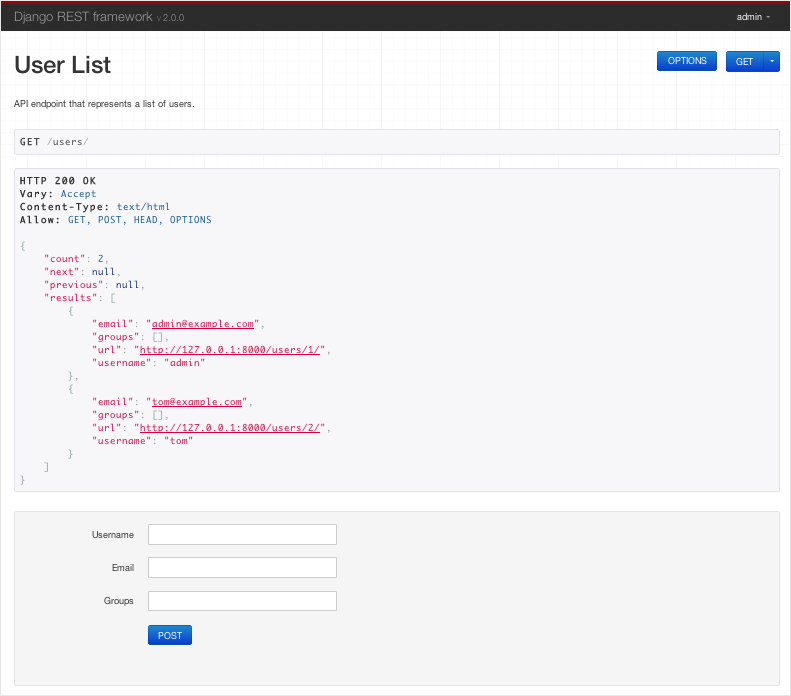
\includegraphics[width=0.8\textwidth]{images/drf-browsable}
	\caption{Die Browsable API}
\end{figure}

\subsection{Sicherheit}

Durch die Einführung einer netzwerkfähigen Schnittstelle werden neue
System-Architekturen möglich (siehe Abschnitt \ref{analyse:architekturen}). Die
strongTNC Komponente muss nicht mehr auf derselben Plattform wie die übrige
strongSwan Infrastruktur betrieben werden.

Für die neugeschaffenen Kommunikationspfade ist Sicherheit nun ein wichtigeres
Thema als zuvor, zumal die Kommunikation von nun an auch über ein Netzwerk
erfolgen kann. Durch die stärkere Exponierung der Schnittstellen werden diese
auch ein potentielles Angriffsziel. Bei der Datenübertragung soll einerseits die
Vertraulichkeit und Integrität der Daten gewährleistet sein, andererseits sollte
durch entsprechende Authentisierungs- und Authorisierungs-Mechanismen der
Zugriff nur für vertrauenswürdige Clients möglich sein. \\ Die adäquate
Verwendung von Transport Layer Security (TLS) würde diese Anforderungen bereits
erfüllen.  Das grosse Risiko hierbei ist jedoch, dass die Verantwortung der
korrekten Umsetzung aus den Händen der Schnittstelle an den Anwender übergeht.
Damit kann die Applikation nicht mehr als grundsätzlich sicher betrachtet
werden, da die sachgemässe Konfiguration des Webservers nicht garantiert werden
kann\cite{owasp2013a5}. Eine optimale Umsetzung würde daher vorsehen,
Sicherheitsaspekte so in die Applikation zu integrieren, dass die Kommunikation
ohne entsprechende Sicherheitsmassnahmen nicht möglich ist. Im Folgenden sollen
mögliche Authentisierungs- und Authorisierungs-Varianten aufgezeigt und deren
Vor- und Nachteile besprochen werden.

\begin{description}

\item [HTTP Basic / Digest] Diese Lösung ist einfach zu implementieren, bedingt
aber den Einsatz von TLS, da sonst Authentisierungsdaten im Klartext übermittelt
werden. Das Protokoll sieht keine Integritätsprüfung und Datenverschlüsselung
vor.

\item [OAuth 1.0a / OAuth 2.0] OAuth ist sehr komplex, das macht es schwierig,
den Standard sicher zu implementieren. Gerade OAuth 2.0 war in der Vergangenheit
harscher Kritik ausgesetzt\cite{hammer2012, homakov2013}. Zudem bietet OAuth 2.0
nur Authorisierung, keine Authentisierung. OAuth 1.0a wäre eine gangbare Lösung,
allerdings werden die meisten der Features von OAuth in der strongTNC API gar
nicht benötigt.

\item [HTTP Signatures] Dieses Verfahren verwendet zusätzliche HTTP Header, um
Signaturen zu übertragen. Die Authentisierung erfolgt anhand einer geleisteten
Signatur. Somit kann die Integrität und Authentizität der übertragenen Daten
gewährleistet werden. Der IETF Standard~\cite{httpsignatures2014} befindet sich allerdings noch im
Entwurfsstadium.

\end{description}

\subsubsection{Implementation} Aus zeitlichen Gründen konnte die nahtlose
Integration von Sicherheitsfeatures in die Schnittstelle nicht umgesetzt werden.
Anstelle wurde Session basierte Authentisierung und HTTP Basic Authentisierung
umgesetzt. Wir empfehlen zudem ausdrücklich, TLS zu verwenden. Um die
Konfiguration von TLS mit Apache zu erleichtern, haben wir eine ausführliche
Deployment Dokumentation verfasst (Abschnitt \ref{anhang:deployment-manual}).
Darin sind unter anderem empfohlene Cypher-Suites, die Aktivierung von
Strict-Transport-Security und eine Anleitung zum Erstellen serverseitiger
Zertifikate enthalten.

\subsubsection{Empfehlung} Falls sich der HTTP Signatures Draft zu einem
Standard durchsetzt, empfehlen wir dessen Implementation mit zusätzlicher
Verwendung von TLS. Obwohl HTTP Signatures ohne TLS verwendet werden können,
weist das HTTP Protokoll verschiedene
Verletzlichkeiten\cite{httpsecconsiderations2014} auf, die durch TLS behoben
werden.
